% begin Chapter ResearchMethodology

\chapter{Research Methodology}
\label{chapter-ResearchMethodology}

\paragraph{ } In Chapter~\ref{chapter-LitReview} we discussed the theoretical basis of scheduling and the planning process of a public transport system. We also analyzed the current literature related to the various stages of the planning process (i.e.:timetabling, vehicle and crew scheduling and crew rostering). Furthermore, in Chapter~\ref{chapter-Introduction} we discussed the background of the present system and the problems associated with the current bus scheduling process as well as the bus transport system as a whole. This chapter will detail the research methodology that was followed during this research project.

The main research objective was to find a solution to help all the stakeholders involved in the public transportation system. In order to do so, people in the scheduling process of the transport system as well authoritative persons in charge of regulating the service were interviewed. In particular, the NTC and the WP RPTA was contacted and several relevant people were interviewed to understand the system \& the service and to ascertain the current problems of the system. A list of persons interviewed have been noted below.

\begin{itemize}
\item Mr. Pradeep Fernando - Head of the GPS Tracking and Monitoring Unit, National Transport Commission.
\item Mr. Dhanushka - Team Member, GPS Tracking and Monitoring Unit, National Transport Commission.
\item Mr. Muditha Navaratne - Timetable Unit of the National Transport Commission.
\item Mr. K.A.R.A. Ranjith - Operations Manager, Western Province Passenger Transport Authority.
\item Mr. Mahesh Nishan - Scheduling Officer, Western Province Passenger Transport Authority.
\item Mr. Theja Athukorala - Scheduling Officer, Western Province Passenger Transport Authority.
\end{itemize}

After the interviews were carried out, an idea of the transportation system and its issues began to emerge. It was then that a pilot route survey was conducted. Details of the survey is mentioned in the following section.

\section{Pilot Route Survey}

\paragraph{ } The bus route chosen for the study is the 177 bus route that runs between Kolpetty and Kaduwela. The route segment between Kolpetty and Rajagiriya was taken into consideration when collecting the data. It is a high value route and is graded as "A+" in a scale of A+, A, B, C by the WP RPTA based on the passenger demand and importance of the route. Additionally, it has buses that are consistently overcrowded and commuters complain about it frequently. Buses on the route are also prone to loitering and many complaints are received regarding this issue making it a perfect candidate to carry out the pilot route survey.

There are 49 buses in in the normal fleet in total with 35 in daily operation. All buses have the capacity to carry around 45 passengers (seated) on average. The route also has Air Conditioned (AC) buses but we will not be considering the AC buses in our data gathering.

\subsection{Gathering the Data}

\paragraph{ } Data was collected by physically traveling in the bus at various times and manually counting the number of passengers that get on and off the bus. This provided information about the passenger demand and load situations in the bus. The time at which the bus arrives and departs each bus stop was also observed and recorded. The time spent at each bus stop was calculated using this data. If the bus loiters at a certain bus stop, the amount of time the driver spends loitering was also recorded.

The data was gathered in this manual way because there is no automated data gathering mechanism currently in place for the private bus system in the Western Province. Further elaboration on automated data gathering and a brief description of the current state of affairs are mentioned in the following section.

As mentioned previously, the current data gathering is done manually by the schedulers at the WP RPTA. The implementation of an ADCS has not been carried out yet due to the reasons mentioned earlier in the chapter. Therefore, the problem remains, how can the data be collected in order to aid in the scheduling and timetabling activities of the RPTA.

The data that is required for the schedulers is the Vehicle Location data and the Passenger Demand data. The former could be obtained by using just a few GPS tracking devices such as the ones the NTC uses in their system, which are fixed temporarily to a few buses. The problem the schedulers face currently is that they have to physically travel in the buses to collect the data. Alternatively, they could use a few (3 or 4) devices to temporarily track the selected buses for the purposes of the survey freeing the need for the schedulers to travel in the buses physically themselves and gather the data. The devices don't have to be fixed permanently onto the buses, just when the survey is being conducted so that the data can be gathered on its movements.

Gathering of the Passenger Demand data is a little more trickier. Passenger Demand is basically a reflection of the number of people that travel in a bus and details of where they get on and off the bus. This could be achieved by counting the number of tickets issued and analyzing the ticketing data. This method however, has a major drawback. It assumes that all commuters are issued a ticket which may not always be the case. Also, not all buses currently have Electronic Ticketing Machines which is an obstacle. The fact that it is not compulsory for the private buses in the WP plying on intra-provincial routes to have Electronic Ticketing Machines is also a major disadvantage to this method. In conclusion, it is clearly evident that reform and stricter regulation of the service is required in order to improve it.

Section~\ref{GatheredData} displays a sample of the data that was gathered during the pilot route survey. The data confirms what most commuters complain about on a regular basis, that the bus loitering is a problem that needs to be dealt with. The survey data also implied that Loitering adds to the problem of overcrowding buses which results in increased dissatisfaction by the commuters.

\subsection {Gathered Data}
\label {GatheredData}

\paragraph{ } Listed below is a sample of the data that was collected. The full list of data is available under Appendix~\ref{appendix-CompleteSetOfData}.

\begin{itemize}

\item Trip Number: 1
\begin{itemize}
\item Date: 23/5/2013
\item Departure Time: 15.40pm
\item Departure Place: Kolpetty
\item Table~\ref{table-trip1-BoardingAndAlighting} and~\ref{table-trip1-LoiterTime}
\end{itemize}
\begin{table}[h!]
\centering
\begin{tabular}{|l|r|r|r|r|}
\hline
Bus Stop & Boarded & Alighted & Net Gain & On Board \\
\hline
 & & & & 0 \\
Kolpetty Depot	&11	&0	&11	&11\\
Supermarket	&10	&0	&10	&21\\
Alwis Place	&7	&0	&7	&28\\
Library	&3	&6	&-3	&25\\
SLTA	&0	&2	&-2	&23\\
\rowcolor[gray]{0.7}
Museum	&1	&0	&1	&24\\
Nelum Pokuna	&2	&2	&0	&24\\
\rowcolor[gray]{0.7}
Alexandra Roundabout	&5	&0	&5	&29\\
Asha Central	&2	&1	&1	&30\\
Wijerama	&4	&0	&4	&34\\
Borella	&2	&5	&-3	&31\\
Devi Balika	&1	&1	&0	&31\\
Castle Street	&1	&0	&1	&32\\
Ayurveda	&2	&6	&-4	&28\\
Rajagiriya	&25	&5	&20	&48\\
\hline
\end{tabular}
\caption{Boarding And Alighting data for Trip 1}
\label{table-trip1-BoardingAndAlighting}
\end{table}

\begin{table}[h!]
\centering
\begin{tabular}{|l|r|r|r|}
\hline
Bus Stop & Arrival Time (h) & Departure Time (h) & Loiter Time (mins) \\
\hline
Kolpetty Depot	&	&15.40	&0\\
Supermarket	&15.44	&15.45	&1\\
Alwis Place	&15.46	&15.46	&0\\
Library	&15.48	&15.49	&1\\
SLTA	&15.50	&15.51	&1\\
Nelum Pokuna	&15.52	&15.53	&1\\
Asha Central	&15.56	&15.56	&0\\
Wijerama	&15.58	&15.58	&0\\
Borella	&16.08	&16.09	&1\\
Devi Balika	&16.11	&16.11	&0\\
Castle Street	&16.14	&16.14	&0\\
Ayurveda	&16.15	&16.16	&1\\
Rajagiriya	&16.18	&16.24	&6\\
\hline
Total Loiter Time & & & 12 mins \\
Duration of Trip & & 44 mins & \\
\hline
\end{tabular}
\caption{Loiter Time Data for Trip 1}
\label{table-trip1-LoiterTime}
\end{table}

\begin {figure} [h!]
\centering
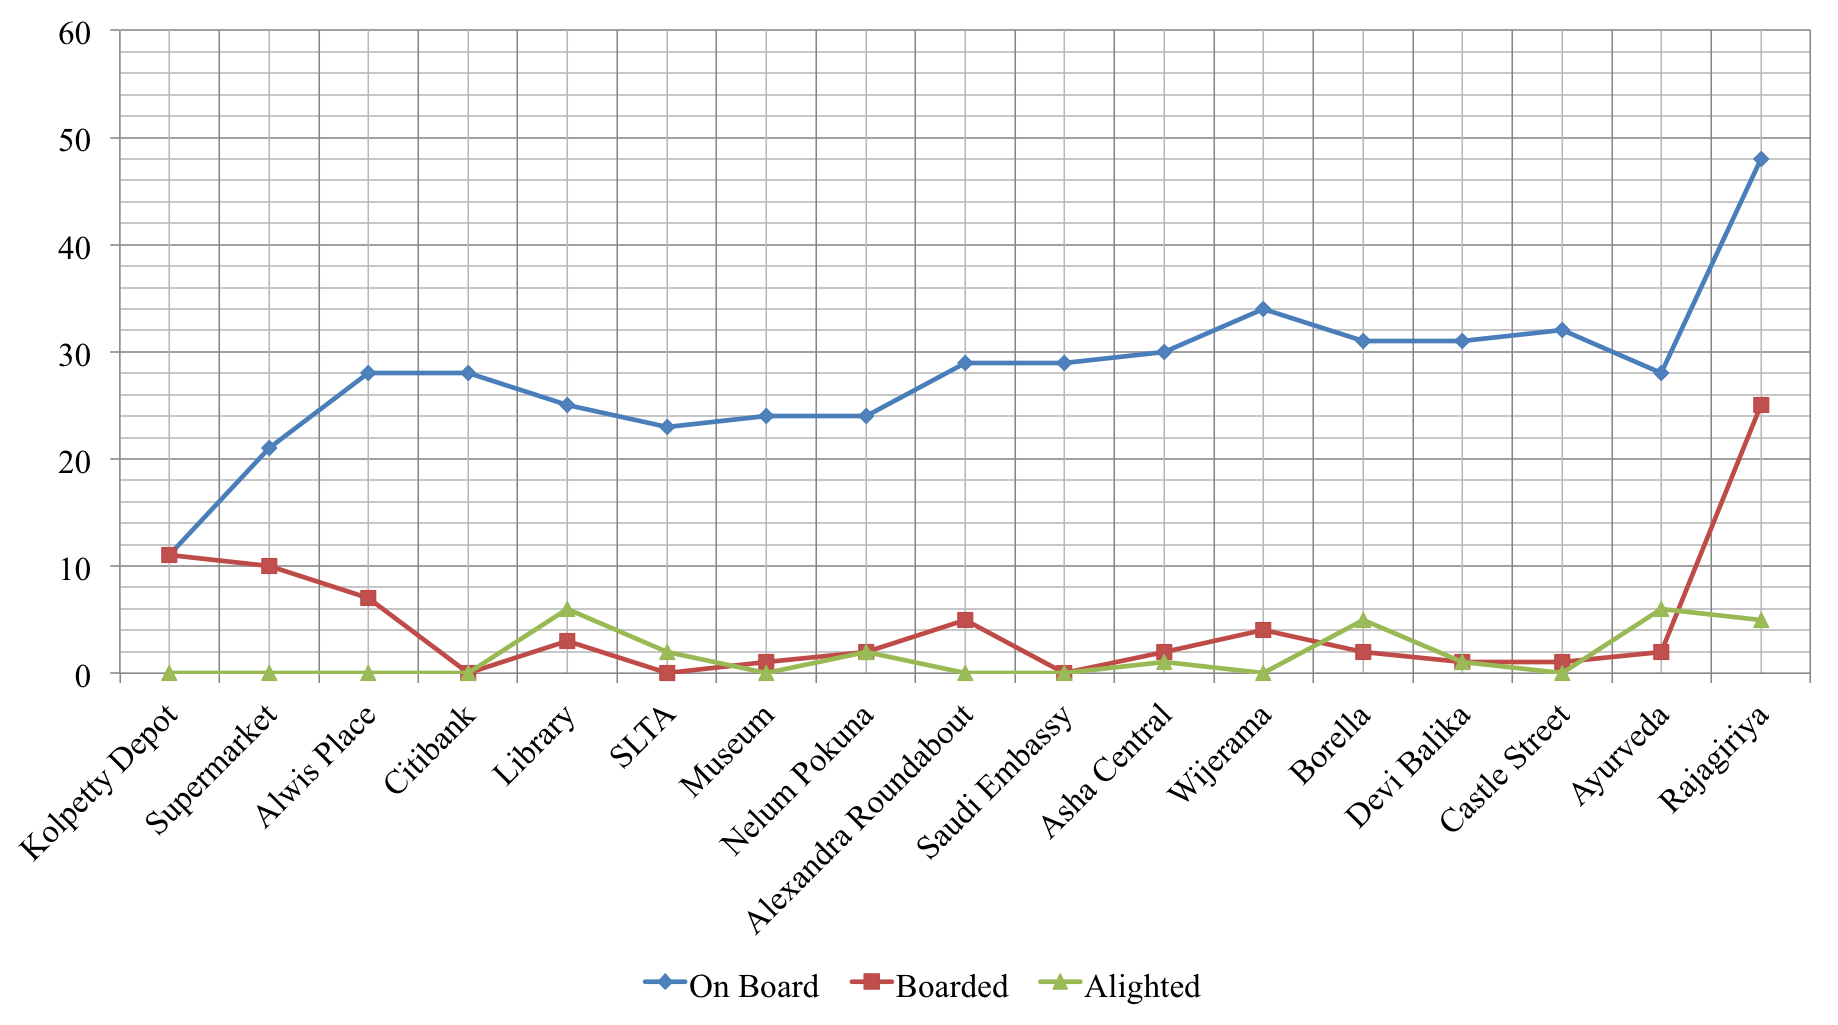
\includegraphics[scale=0.5]{passengerLoadData-Trip1}
\caption [Graph - Passenger Load Fluctuations - Trip 1] {Graph - Passenger Load Fluctuations - Trip 1}
\label {image-passengerLoadData-Trip1}
\end {figure}

\begin {figure} [h!]
\centering
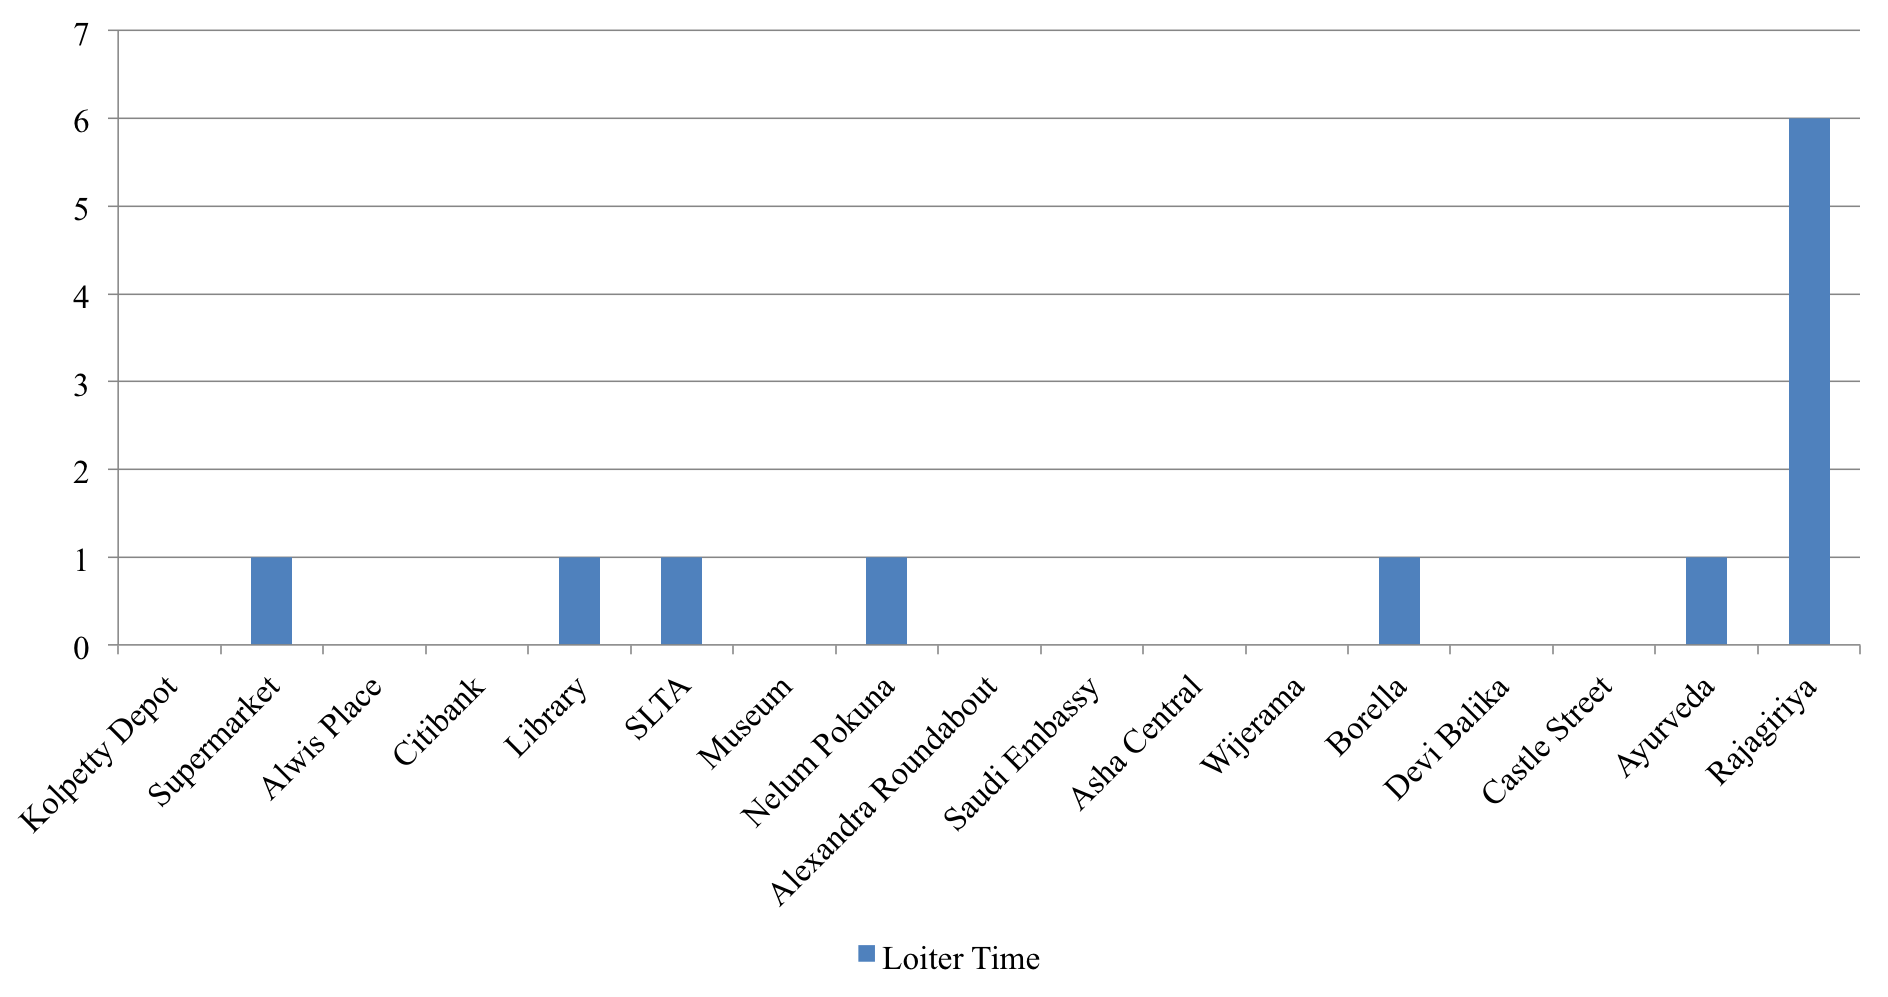
\includegraphics[scale=0.5]{loiterTimeData-Trip1}
\caption [Graph - Bus Loiter Time Data - Trip 1] {Graph - Bus Loiter Time Data - Trip 1}
\label {image-loiterTimeData-Trip1}
\end {figure}

\end{itemize}


\newpage

\section {Stakeholder Analysis}
\label {StakeholderAnalysis}

\paragraph{} The stakeholders of this Public Transport System are illustrated in Figure~\ref{image-stakeholdersDiagram}.

\begin {figure} [h!]
\centering
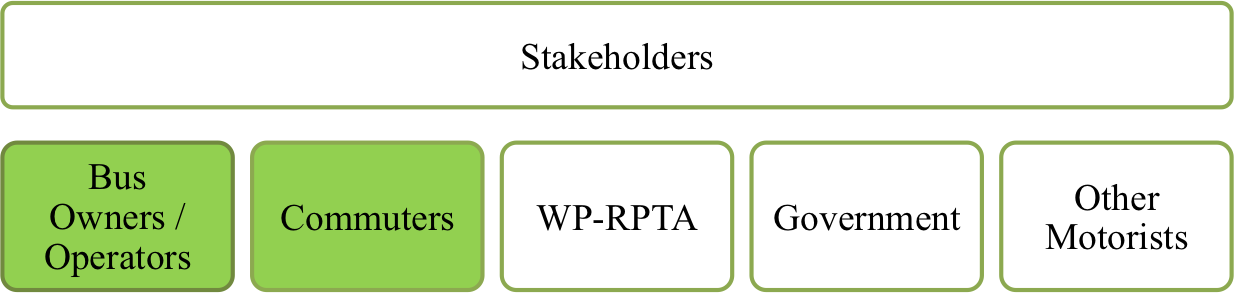
\includegraphics[scale=0.75]{stakeholdersDiagram}
\caption [Stakeholders Diagram] {Stakeholders Diagram}
\label {image-stakeholdersDiagram}
\end {figure}

\paragraph{} The most prominent stakeholders in this system are the Commuters and the Bus Owners/Operators. These 2 serve as the Demand and Supply sides of the economic equation respectively. The conflicting requirements of these two parties are illustrated in Figure~\ref{image-mainStakeholdersDiagram}.

\begin {figure} [h!]
\centering
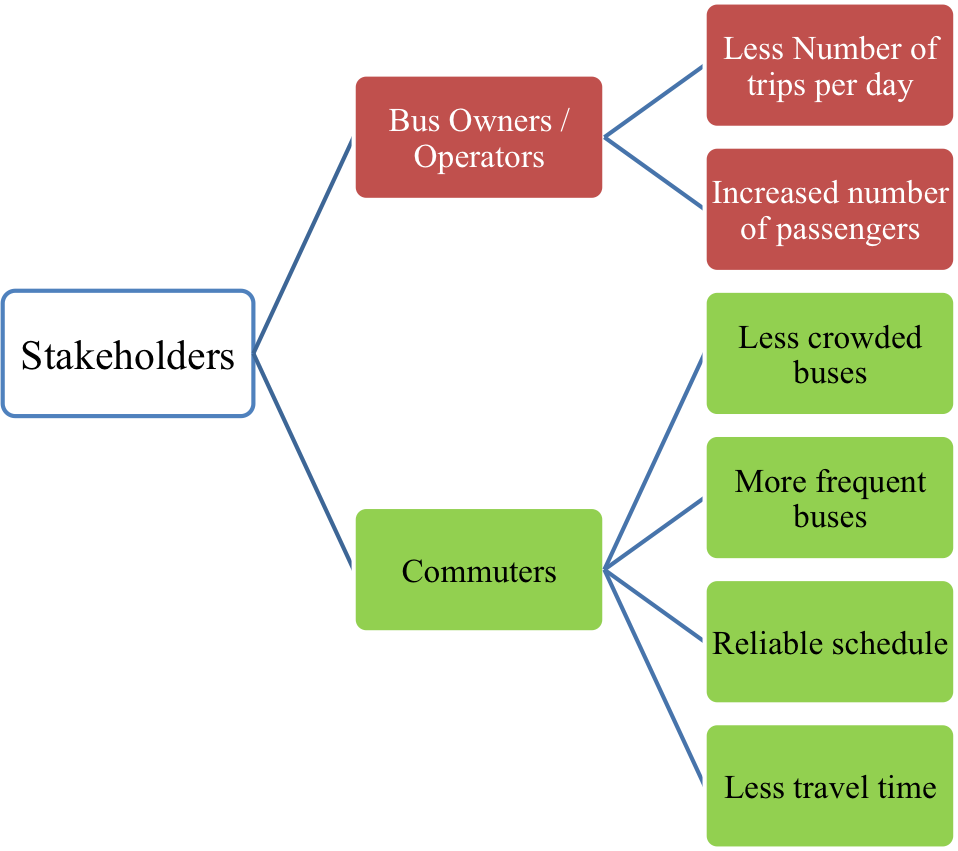
\includegraphics[scale=0.7]{mainStakeholdersDiagram}
\caption [Requirements of Main Stakeholders] {Requirements of Main Stakeholders}
\label {image-mainStakeholdersDiagram}
\end {figure}

\paragraph{} However, it is the Transport Authority that has the responsibility to keep these two parties happy. Therefore the most important stakeholder of the whole system is the Transport Authority and that is why it is important that a System is implemented that assists the Schedulers in their decision-making process. The workflow of the Scheduling Unit of the WP RPTA is comprised of 3 main stages. They are illustrated in Figure~\ref{image-timetablingProcessSteps}. The proposed Decision Support System,detailed in Chapter~\ref{chapter-ProposedSolution} will have this workflow at its core.

\begin {figure} [h!]
\centering
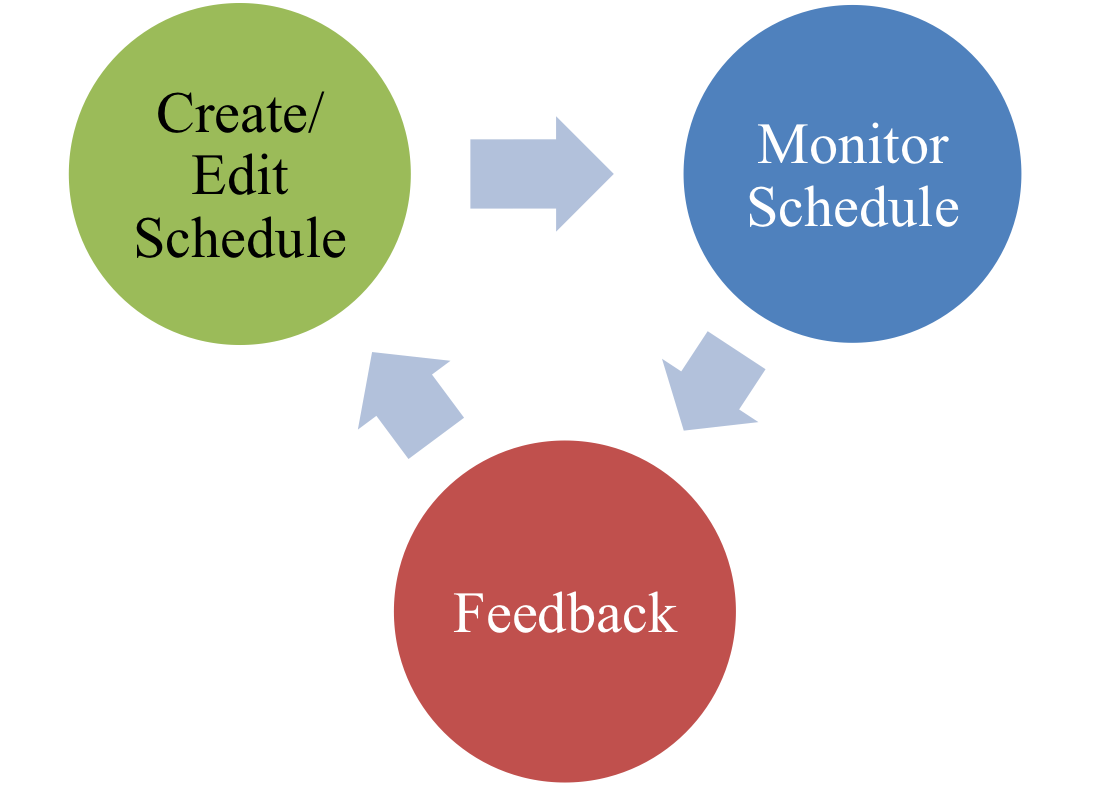
\includegraphics[scale=0.5]{timetablingProcessSteps}
\caption [Stages in the Timetabling Process Flow] {Stages in the Timetabling Process Flow}
\label {image-timetablingProcessSteps}
\end {figure}

\newpage

\section{Possible Alternative Solutions}
\label{section-Alternatives}

\paragraph{} From the contents of the current Chapter, the problems of the current system and transport service are clearly evident. From the Pilot Route Survey that was conducted, the data gathering requirements of the proposed DSS is clear.

Accordingly, possible solutions to these problems were an implementation of a Management Information System or a standalone system to create timetables for the schedulers. However neither of these really addressed all of the issues for all of the stakeholders. Management Information Systems are systems or processes that provide the information necessary to manage an organization effectively \cite{Comptroller1995, TexasAMUni2012}. Although this does accomplish the outcome of better management for the Schedulers, it does little to manage the customer-facing activities. It also focuses on management of the organization instead of aiding in the decision-making process.

Alternatively, a standalone system to merely create timetables and schedules for the bus routes does not solve all of the problems faced. Therefore, the need for a Decision Support System to aid the various stakeholders in their decision-making processes as well as enabling the proper monitoring and regulation of the service is clearly evident. The definition of a Decision Support System and how it relates to the transportation problem has already been discussed in this document. Therefore, in the next Chapter, we will see what the proposed Decision Support System is. This will include the higher-level system architecture, the system features, the main entities \& their relationships and a few screenshots of the prototype that was built for user testing.